
\documentclass[12pt,a4paper,titlepage,oneside]{article}
\usepackage[top=2.5cm, bottom=2cm, left=2.5cm, right=1cm]{geometry} 
% Font, accents
\usepackage[utf8]{inputenc}
\usepackage{fancyhdr}
\usepackage[T1]{fontenc}
\usepackage{times}     
% Interactive index
\usepackage{hyperref}
% Spanish titles
\usepackage[spanish]{babel}
% Attached files
\usepackage{attachfile}
\attachfilesetup{
  icon = Paperclip
}
% Fix curly verbatim apostrophes
\usepackage{upquote,textcomp}
% Make lists without bullets
\renewenvironment{itemize}{
 \begin{list}{}{
  \setlength{\leftmargin}{1.5em}
 }
}{
 \end{list}
}



%Customize things
\usepackage[margin=0pt,font=small,labelfont=bf]{caption}
\usepackage{graphicx}
\usepackage[usenames,dvipsnames]{xcolor}

% Sections and subsections colors
\usepackage{titlesec}
\titleformat{\section}
{\color{Blue}\normalfont\Large\bfseries}
{\color{Blue}\thesection}{1em}{}
\newcommand{\sectionbreak}{\clearpage}


% Document properties
\title{Facultad de Ingeniería\\Análisis de la información (75.09)}
\date{\today}
\hypersetup{
  colorlinks = true,
  urlcolor=blue,
  pdflang = es,
  pdfauthor = {Federico Farina},
  pdfproducer = {Federico Farina},
  pdfcreator = Texmaker,
  pdftitle = {Análisis de la información},
}

\begin{document}
   % code start
    \fancyhead[LE]{\leftmark} 
    \fancyhead[RO]{\rightmark} 
    \fancyhead[L]{Análisis de la información}
    \fancyhead[R]{IR-TOUR}    
    \renewcommand{\headrulewidth}{0.4pt} 
    \renewcommand{\footrulewidth}{0pt}
    % code end

    % set pagestyle to use fancy header and footer
    \pagestyle{fancy}


 \maketitle
  \setcounter{page}{1}
  \pagenumbering{roman}
  \tableofcontents

\newpage{}
\pagenumbering{arabic}
\setcounter{page}{1}

\section{Enunciado}

La Licenciada en Turismo Irma Josefina B. es la propietaria de la agencia IR-TOUR, la cual se dedica a organizar tours alrededor del mundo.
Cuando un cliente contrata un tour, el vendedor confecciona el contrato con las condiciones del servicio y una chequera de pagos con el detalle de las fechas e importes de las cuotas.
En la fecha de vencimiento de cada cuota, el cliente la abona en Tesorería. Este podrá abonarla en efectivo o con tarjeta de crédito. La empleada revisa los importes y sella el talón que corresponda a la cuota. Si paga con tarjeta de crédito chequea la misma telefónicamente y si todo es correcto, confecciona el cupón de pago respectivo y le entrega el original. Cuando un cliente va a efectuar el tour, retira de la agencia un talonario con todas las órdenes de servicio para los hoteles, excursiones y pasajes correspondientes. El vendedor antes de entregarle este talonario procede a corroborar que el cliente tenga todas sus cuotas abonadas mediante la chequera sellada. Una vez concretada la operación los vendedores deberán avisarle urgentemente a Irma para que ella comunique a las empresas intervinientes los pasajeros del tour.Irma es la encargada de efectuar las reservas hoteleras, contratar excursiones y reservar vuelos y micros, puesto que es ella la que tiene los contactos. Estas empresas pueden comunicar modificaciones (cambios, demoras y anulaciones) para las contrataciones efectuadas. Una vez que Irma contrato nuevos servicios y negoció las modificaciones de reservas ya existentes se las comunica a sus vendedores. Éstos, en base a las instrucciones de Irma deberán armar los nuevos tours y además comunicar a los clientes dichas novedades para proceder a reconfirmar los pedidos, cambiarlos, efectuar anulaciones y devolución de los pagos efectuados por los clientes.
Asimismo, todos los fines de mes se envía a los clientes regulares las promociones y ofertas de IR-TOUR en diversas modalidades: correo, fax, internet, etc.


\section{Modelo de negocios}

\subsection{Propósito}
Modelizar las actividades que se realizan al organizar los tours de una agencia de viaje. 
Las actividades son: organizar y vender paquetes turísticos, realizar contratos con los clientes, confeccionar talonarios, realizar reservas hoteleras, excursiones  y vuelos. A su vez se tiene como objetivo informar a los clientes de promociones y ofertas disponibles y el posterior cobro y contratación de los servicios.


\subsection{Alcance}

\begin{itemize}
\item[•] Confección de contratos
\item[•] Recepción de pagos.
\item[•] Confección de talonarios
\item[•] Armado de tours
\item[•] Reservacion de hoteles, excursiones, vuelos, micros
\item[•] Publcidad
\item[•] Promociones
\end{itemize}



\subsection{Hipótesis y supuestos}

\begin{itemize}
\item[•] Pago de tours en una única moneda pesos argentinos, efectivo o tarjeta.
\item[•] Pagos en cuotas sin interés.
\item[•] El pago de las cuotas es mensual.
\item[•] Pagos del 1 al 10 de cada mes.
\item[•] Devoluciones o cancelaciones de paquetes turísticos con 30 días de anticipación.
\item[•] Los hoteles, vuelos y excursiones están sujetos a la disponibilidad de los mismos y pueden ser modificados  tratandose siempre de respetar las fechas y categorías elegidas por el cliente.
\item[•] A la primer cuota paga, la gerencia realiza las contrataciones/reservas pertinentes.
\item[•] La gerencia puede realizar todo tipo de cancelación.
\end{itemize}

\newpage
\subsection{Diagrama de actividad}

Diagramas de actividad
\bigskip

\begin{figure}[htb]
\centerline{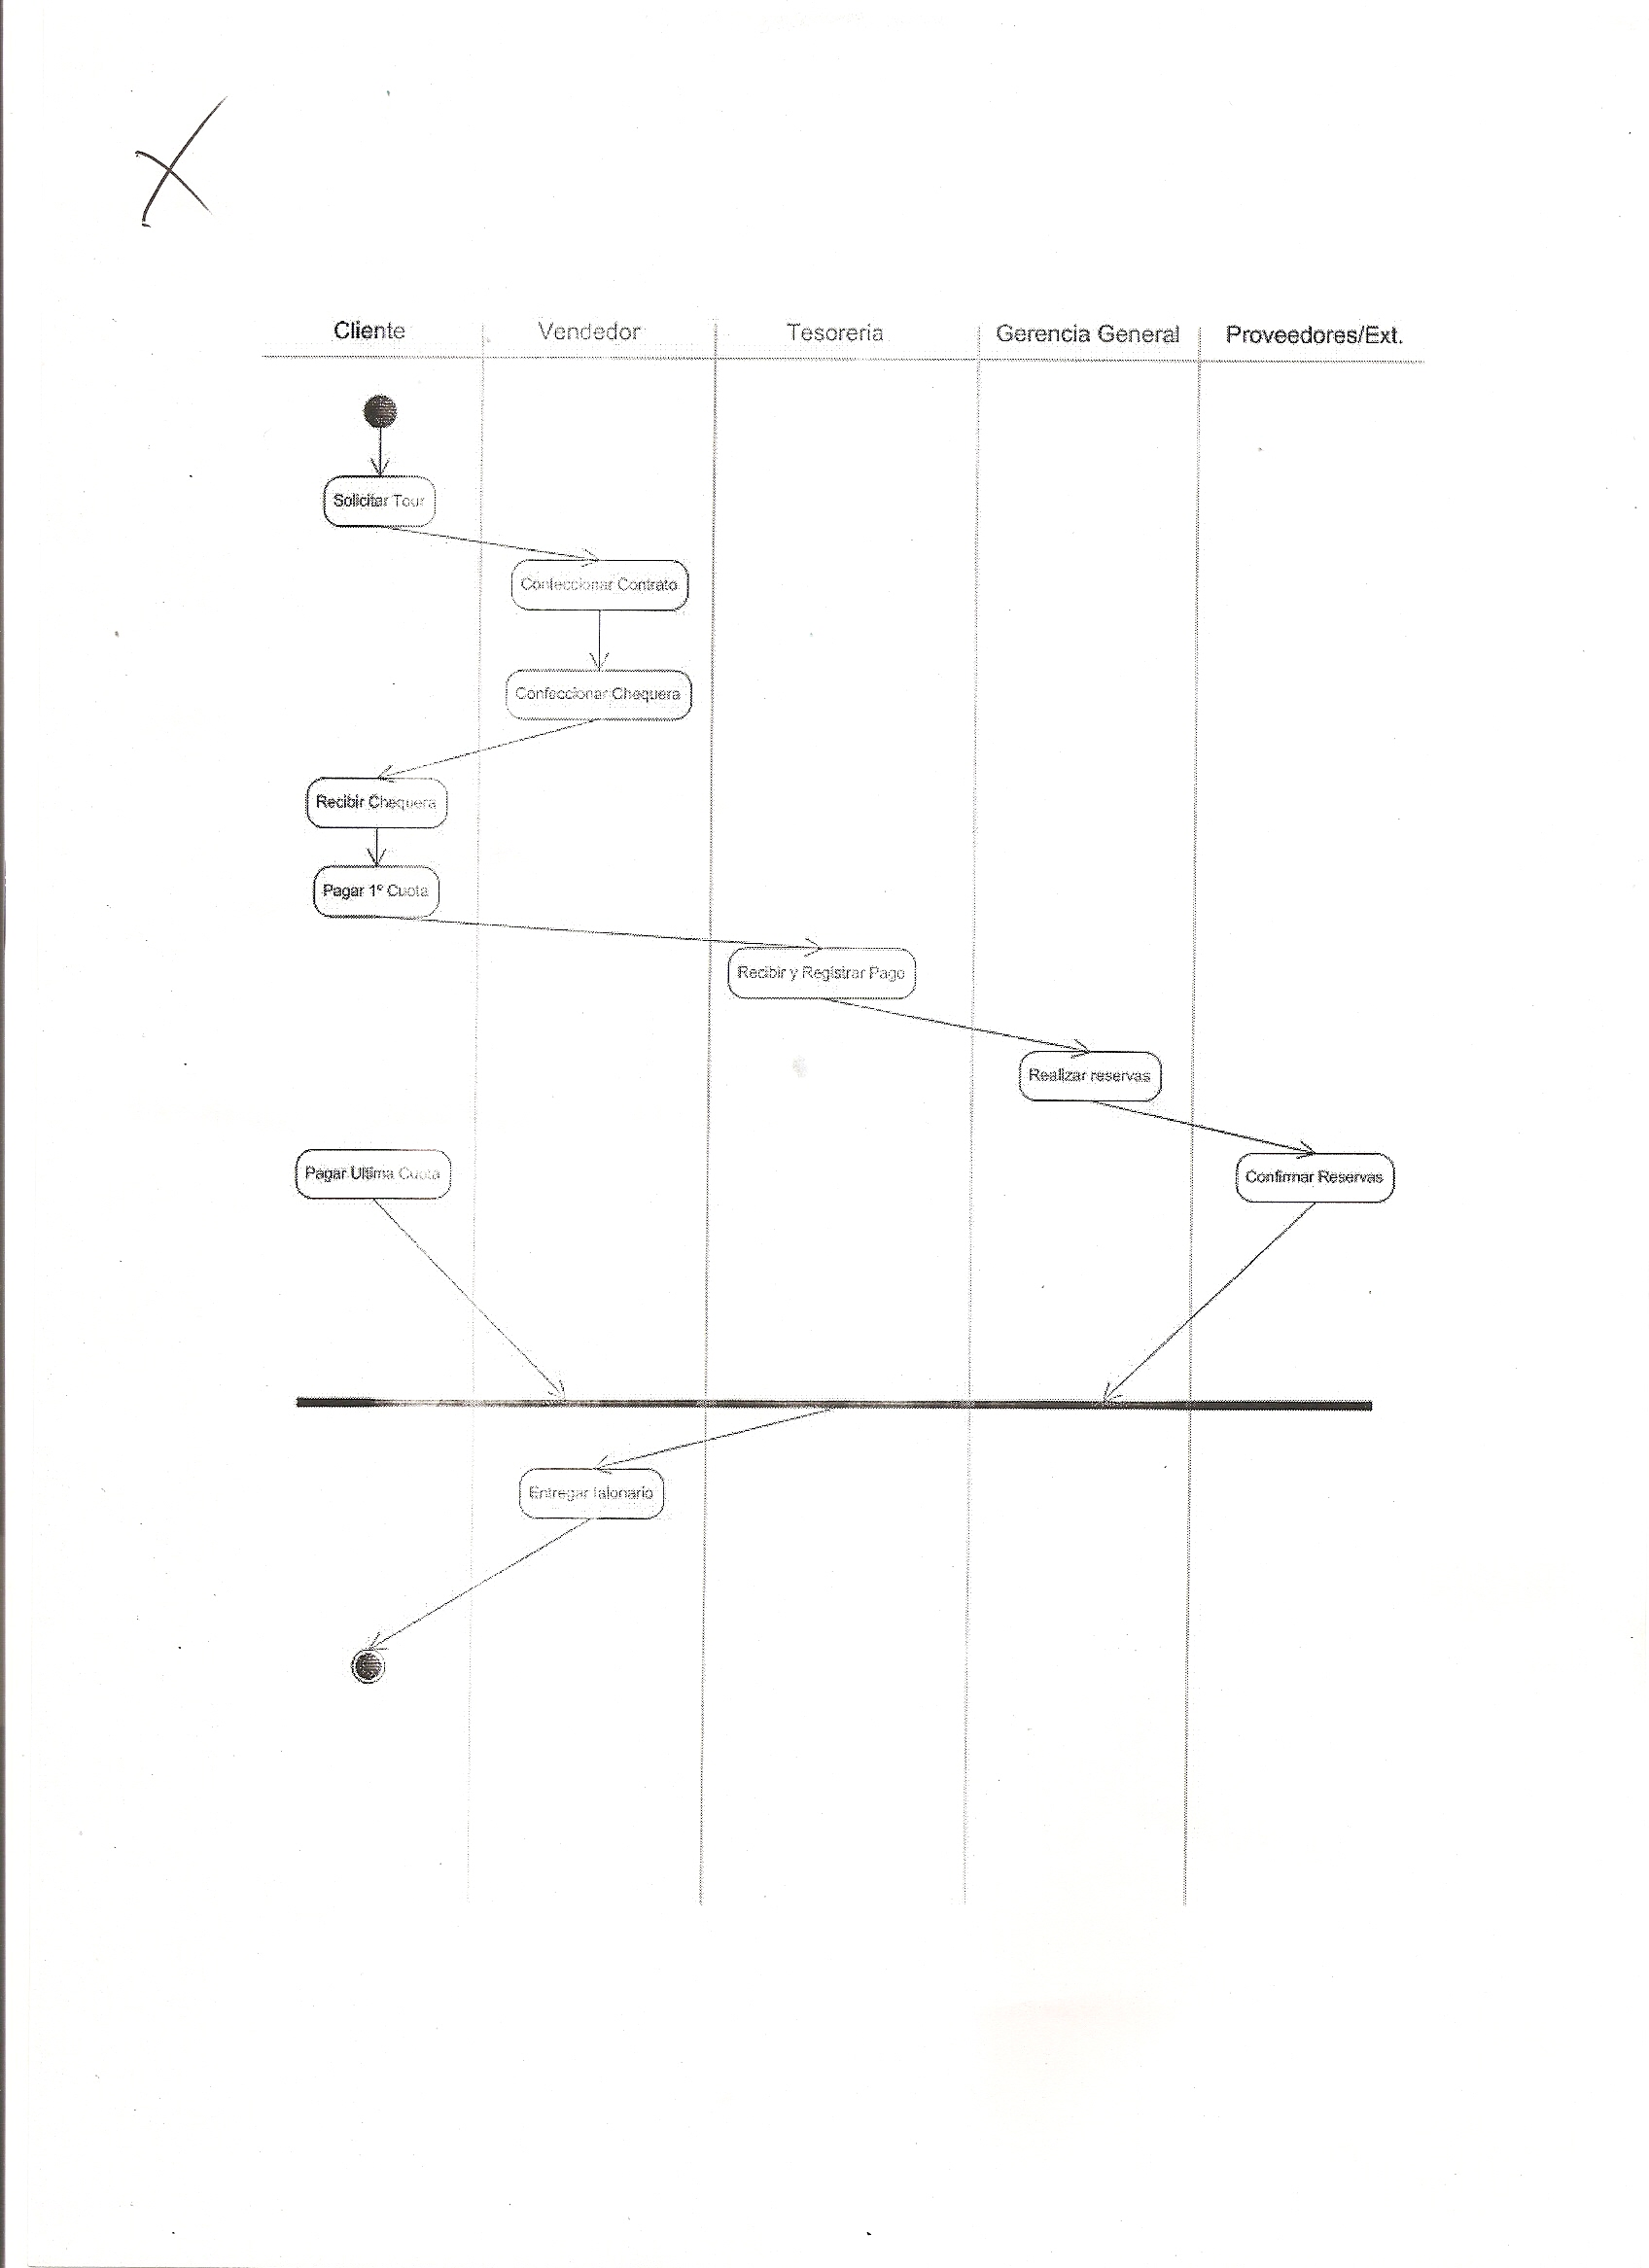
\includegraphics[width=0.8\textwidth]{escenario1}}
\label{fig:celda}
\end{figure}

\begin{figure}[htb]
\centerline{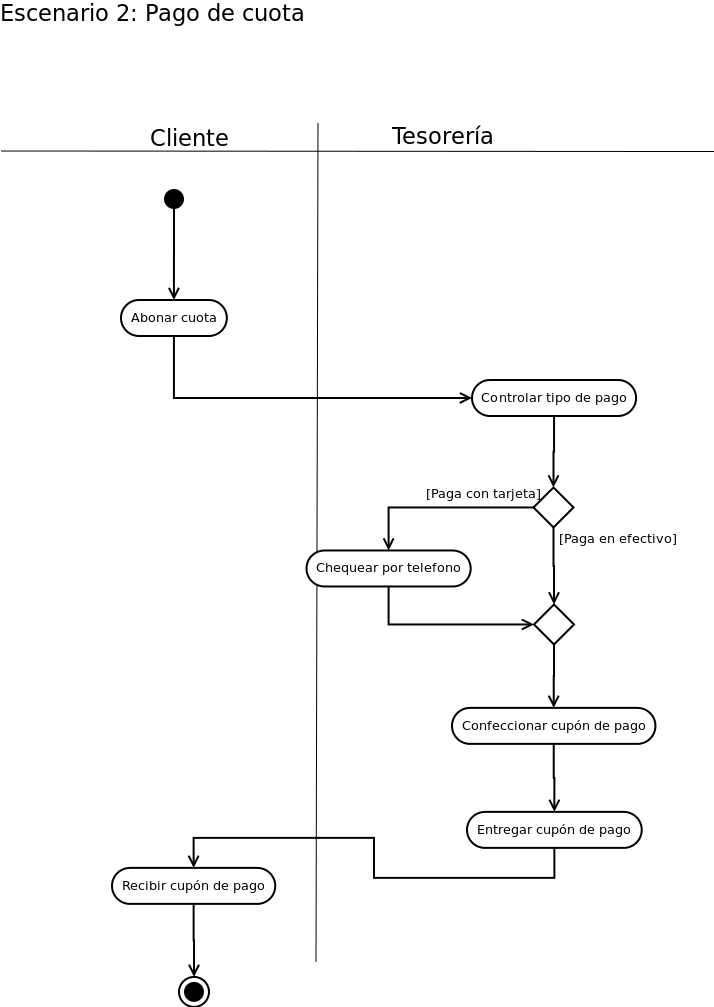
\includegraphics[width=0.9\textwidth]{escenario2}}
\label{fig:celda}
\end{figure}

\begin{figure}[htb]
\centerline{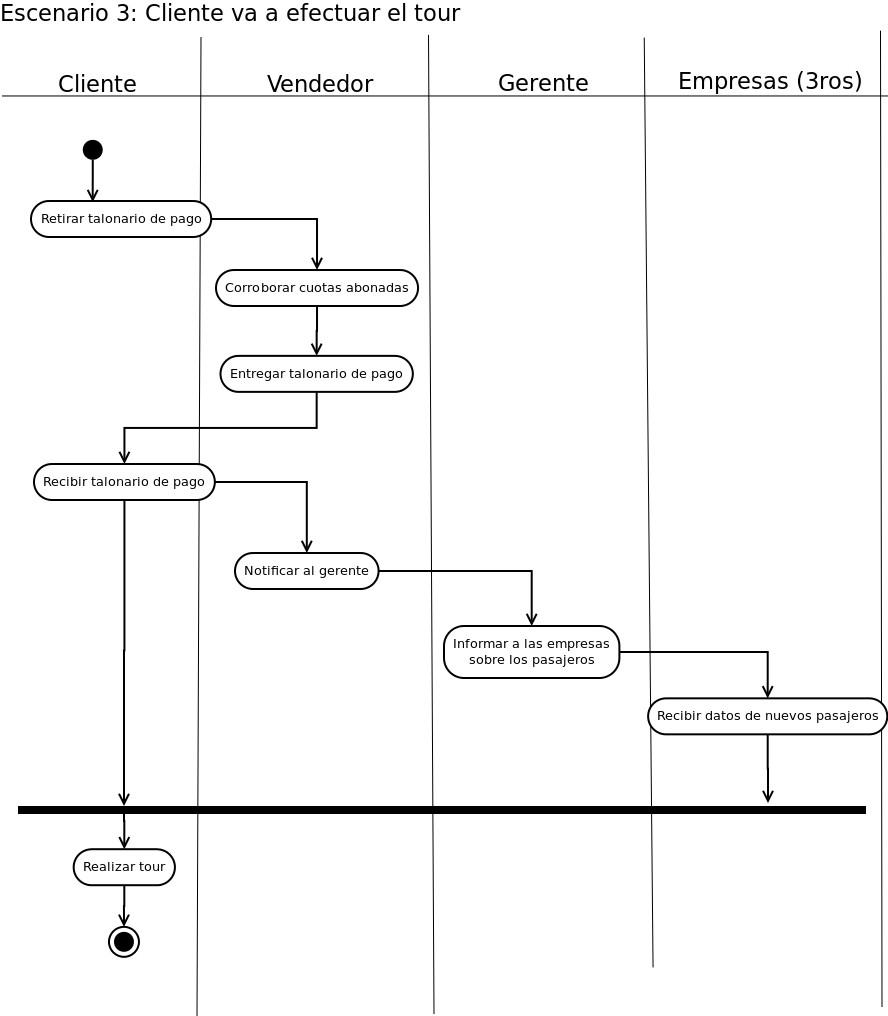
\includegraphics[width=0.9\textwidth]{escenario3}}
\label{fig:celda}
\end{figure}

\begin{figure}[htb]
\centerline{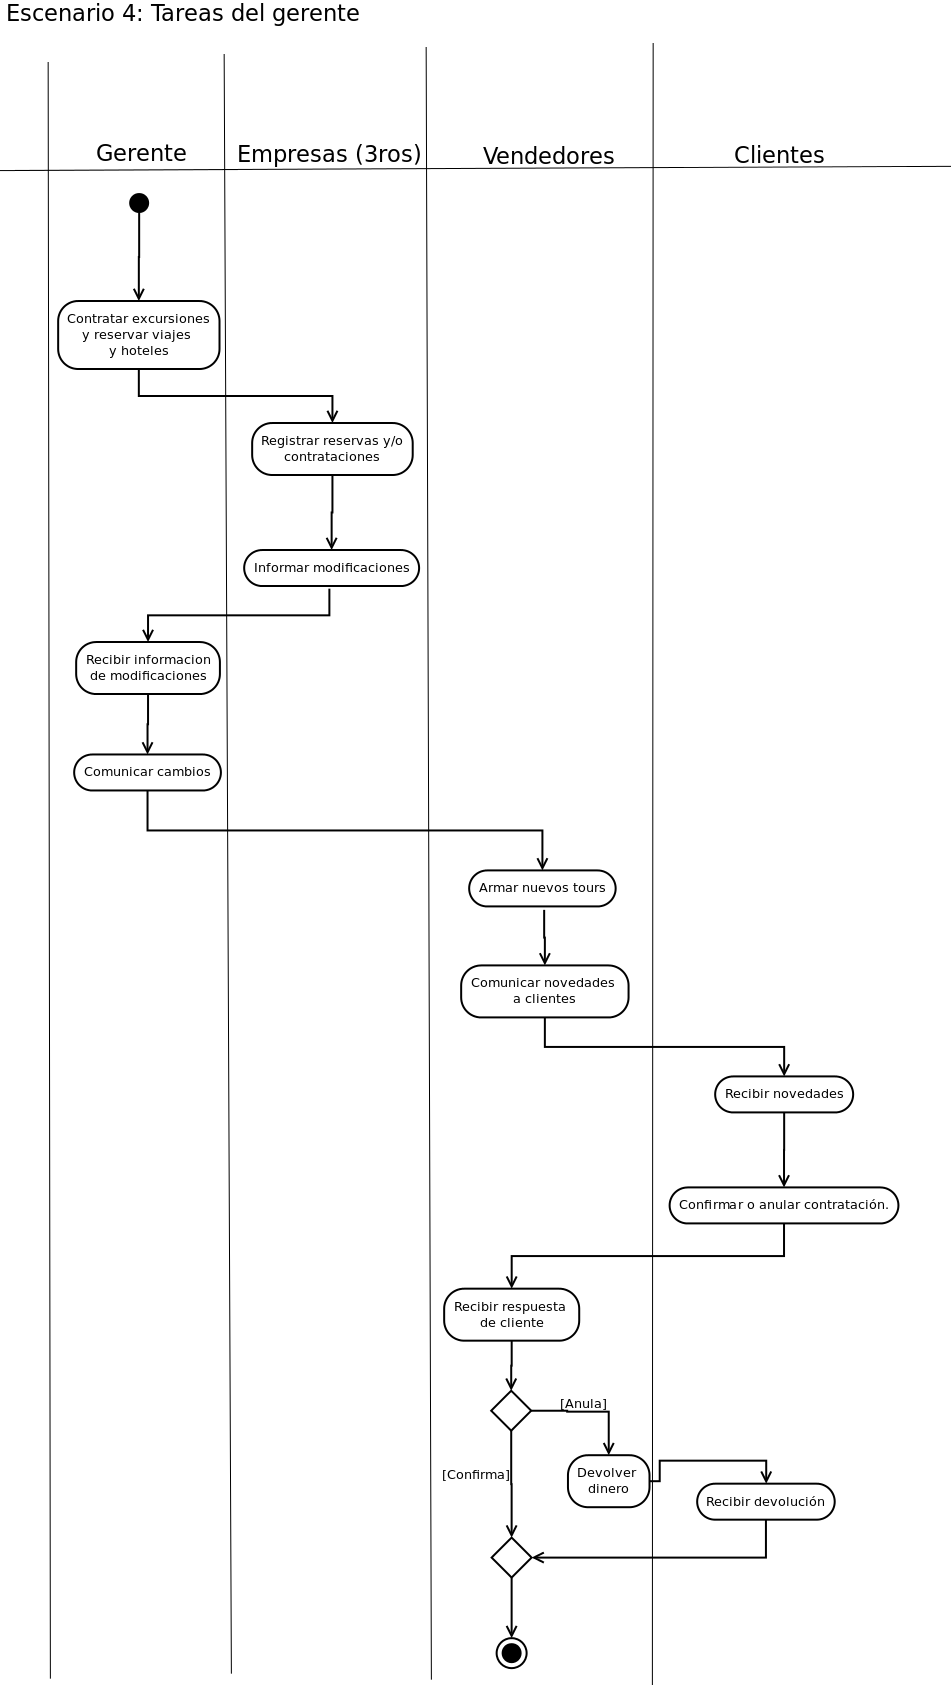
\includegraphics[width=0.8\textwidth]{escenario4}}
\label{fig:celda}
\end{figure}


\section{Modelo de casos de uso}

Modelo de casos de uso 

\subsection{Actores}


\vspace*{1.5cm}

\begin{minipage}[b]{0.2\linewidth}\centering
	
\includegraphics[height=2cm]{actor_cliente}
\end{minipage}
\begin{minipage}[b]{0.8\linewidth}\centering
	\begin{flushleft}
	Persona que acude a la agencia para contratar un tour. \\
	\end{flushleft}
\end{minipage}


\vspace*{1.5cm}

\begin{minipage}[b]{0.2\linewidth}\centering
	
\includegraphics[height=2cm]{actor_vendedor}
\end{minipage}
\begin{minipage}[b]{0.8\linewidth}\centering
	\begin{flushleft}
	Persona encargada de confeccionar contratos con el cliente, armar tours, comunicarse con el cliente y efectuar anulaciones. \\
	\end{flushleft}
\end{minipage}

\vspace*{1.5cm}


\begin{minipage}[b]{0.2\linewidth}\centering
	
\includegraphics[height=2cm]{actor_propietario}
\end{minipage}
\begin{minipage}[b]{0.8\linewidth}\centering
	\begin{flushleft}
	Persona propetaria de la agencia, realiza reservas hoteleras, contrata excursiones y reserva vuelos y micros. Informa a los vendedores sobre las contrataciones de servicios y modificaciones de reservas. \\
	\end{flushleft}
\end{minipage}


\vspace*{1.5cm}


\begin{minipage}[b]{0.2\linewidth}\centering
	
\includegraphics[height=2cm]{actor_tesoreria}
\end{minipage}
\begin{minipage}[b]{0.8\linewidth}\centering
	\begin{flushleft}
	Recibe los pagos de cuotas de los clientes. \\
	\end{flushleft}
\end{minipage}

\vspace*{1.5cm}

\begin{minipage}[b]{0.2\linewidth}\centering
	
\includegraphics[height=2cm]{actor_temporal}
\end{minipage}
\begin{minipage}[b]{0.8\linewidth}\centering
	\begin{flushleft}
	Se encarga de enviar las promociones. \\
	\end{flushleft}
\end{minipage}

\vspace*{1.5cm}


%\begin{minipage}[b]{0.2\linewidth}\centering
%	
\includegraphics[height=2.25cm]{entidadFinanciera}
%\end{minipage}
\begin{minipage}[b]{0.8\linewidth}\centering
	\begin{flushleft}
Entidad que se encarga de las operaciones de validación que involucran la tarjeta de crédito. \\
	\end{flushleft}
\end{minipage}


\vspace*{1.5cm}



\newpage

\subsubsection{Identificación de casos de uso}

\begin{enumerate}
\item Contratar tour
\item Reservar tours
\item Confeccionar y enviar publicidad
\item Pagar cuota
\end{enumerate}


\subsubsection{Desarrollo de casos de uso}

Desarrollo de casos de uso
\\\

\begin{tabular}{| l | p{0.8\linewidth} |} \hline
	\multicolumn{2}{|p{0.8\linewidth}|}{\textbf{Use Case:} 1 Contratar tour} \\ \hline
	\multicolumn{2}{|c|}{} \\ \hline
	\multicolumn{2}{|p{0.8\linewidth}|}{\textbf{Descripci\'on:} Se le entrega un contrato al cliente y  la chequera de pagos.} \\ \hline
	\multicolumn{2}{|p{0.8\linewidth}|}{\textbf{Actores participantes:} Cliente, Vendedor.} \\ \hline
	\multicolumn{2}{|p{0.8\linewidth}|}{\textbf{Pre-condiciones:} El cliente debe haber entregado la documentación necesaria.} \\ \hline
	\multicolumn{2}{|c|}{} \\ \hline
	\multicolumn{2}{|p{0.8\linewidth}|}{\textbf{Flujos}} \\ \hline
	\multicolumn{2}{|p{0.8\linewidth}|}{\textbf{Flujo principal}} \\ \hline
	\multicolumn{2}{|p{0.8\linewidth}|}{\textbf{1} El cliente contrata un tour.} \\ \hline
	\multicolumn{2}{|p{0.8\linewidth}|}{\textbf{2} El vendedor corrobora que la documentación sea correcta.} \\ \hline
	\multicolumn{2}{|p{0.8\linewidth}|}{\textbf{3} El vendedor confecciona el contrato y le entrega la chequera al	cliente.} \\ \hline
	\multicolumn{2}{|p{0.8\linewidth}|}{\textbf{Flujos de excepci\'on}} \\ \hline
	\multicolumn{2}{|p{0.8\linewidth}|}{\textbf{E1} La documentación entregada no es correcta} \\ \hline
	\multicolumn{2}{|p{0.8\linewidth}|}{\textbf{E1.1} El vendedor anula la operación} \\ \hline
	\multicolumn{2}{|p{0.8\linewidth}|}{\textbf{Post-condiciones:} El cliente ahora tiene chequera de pagos y un contrato.}\\ \hline
\end{tabular} \\\\
 \\\\


\begin{tabular}{| l | p{0.8\linewidth} |} \hline
	\multicolumn{2}{|p{0.8\linewidth}|}{\textbf{Use Case:} 2 Reservar tours} \\ \hline
	\multicolumn{2}{|c|}{} \\ \hline
	\multicolumn{2}{|p{0.8\linewidth}|}{\textbf{Descripci\'on:} El propietario hace las reservas para las excursiones, vuelos y hoteles.} \\ \hline
	\multicolumn{2}{|p{0.8\linewidth}|}{\textbf{Actores participantes:} Propietario, Cliente, Vendedor.} \\ \hline
	\multicolumn{2}{|p{0.8\linewidth}|}{\textbf{Pre-condiciones:} El cliente debe tener todas las cuotas pagas} \\ \hline
	\multicolumn{2}{|c|}{} \\ \hline
	\multicolumn{2}{|p{0.8\linewidth}|}{\textbf{Flujos}} \\ \hline
	\multicolumn{2}{|p{0.8\linewidth}|}{\textbf{Flujo principal}} \\ \hline
	\multicolumn{2}{|p{0.8\linewidth}|}{\textbf{1-} El cliente va a la agencia para pedir el talonario de servicio.} \\ \hline
	\multicolumn{2}{|p{0.8\linewidth}|}{\textbf{2-} El vendedor se fija que el cliente tenga todas las cuotas pagas y la chequera sellada.} \\ \hline
	\multicolumn{2}{|p{0.8\linewidth}|}{\textbf{3-} El vendedor comunica al propietario que ya puede efectuar las reservas.} \\ \hline
		\multicolumn{2}{|p{0.8\linewidth}|}{\textbf{4-} El propietario efectua las reservas.} \\ \hline
	\multicolumn{2}{|p{0.8\linewidth}|}{\textbf{Post-condiciones:} El cliente ahora tiene la orden de servicio y se realizaron las reservas pertinentes.}\\ \hline
\end{tabular} \\\\
 \\\\


\begin{tabular}{| l | p{0.8\linewidth} |} \hline
	\multicolumn{2}{|p{0.8\linewidth}|}{\textbf{Use Case:} 3 Confeccionar y enviar publicidad} \\ \hline
	\multicolumn{2}{|c|}{} \\ \hline
	\multicolumn{2}{|p{0.8\linewidth}|}{\textbf{Descripci\'on:} El vendedor envía a los clientes las promociones y ofertas de la agencia.} \\ \hline
	\multicolumn{2}{|p{0.8\linewidth}|}{\textbf{Actores participantes:} Vendedor, Actor temporal.} \\ \hline
	\multicolumn{2}{|p{0.8\linewidth}|}{\textbf{Pre-condiciones:} Se tiene una lista de clientes usuales} \\ \hline
	\multicolumn{2}{|c|}{} \\ \hline
	\multicolumn{2}{|p{0.8\linewidth}|}{\textbf{Flujos}} \\ \hline
	\multicolumn{2}{|p{0.8\linewidth}|}{\textbf{Flujo principal}} \\ \hline
	\multicolumn{2}{|p{0.8\linewidth}|}{\textbf{1} El vendedor envía al cliente las promociones de la agencia por medio de un actor temporal.} \\ \hline
	\multicolumn{2}{|p{0.8\linewidth}|}{\textbf{2} El actor temporal distribuye las promociones.} \\ \hline
	\multicolumn{2}{|p{0.8\linewidth}|}{\textbf{3} El vendedor comunica al propietario que ya puede efectuar las reservas.}\\ \hline
	\multicolumn{2}{|p{0.8\linewidth}|}{\textbf{Post-condiciones:} El cliente está enterado de las útimas novedades de la agencia.}\\ \hline
\end{tabular} \\\\
\\\\\\\\


\begin{tabular}{| l | p{0.8\linewidth} |} \hline
	\multicolumn{2}{|p{0.8\linewidth}|}{\textbf{Use Case:} 4 Mantener Tour} \\\hline
	\multicolumn{2}{|c|}{} \\ \hline
	\multicolumn{2}{|p{0.8\linewidth}|}{\textbf{Descripci\'on:} El propietario modifica tours existentes o ingresa nuevos} \\ \hline
	\multicolumn{2}{|p{0.8\linewidth}|}{\textbf{Actores participantes:} Propietario} \\ \hline
	\multicolumn{2}{|p{0.8\linewidth}|}{\textbf{Pre-condiciones:} -.} \\ 			    \hline
		\multicolumn{2}{|p{0.8\linewidth}|}{\textbf{Flujo principal}} \\ \hline
	\multicolumn{2}{|p{0.8\linewidth}|}{\textbf{1}  El sistema solicita la actividad a realizar: } \\ \hline
	\multicolumn{2}{|p{0.8\linewidth}|}{  Si la actividad es Alta, ejecutar flujo alternativo A1.} \\ \hline
	\multicolumn{2}{|p{0.8\linewidth}|}{  Si la actividad es Baja, ejecutar flujo alternativo A2.} \\ \hline
		\multicolumn{2}{|p{0.8\linewidth}|}{  Si la actividad es Modificación, ejecutar flujo alternativo A3.} \\ \hline
		\multicolumn{2}{|p{0.8\linewidth}|}{  Si la actividad es Salir, terminar caso de uso.} \\ \hline

	\multicolumn{2}{|p{0.8\linewidth}|}{\textbf{Flujos alternativos:}	}\\ 			     \hline
	\multicolumn{2}{|p{0.8\linewidth}|}{\textbf{A1: Alta de Tour}} \\ \hline
	\multicolumn{2}{|p{0.8\linewidth}|}{\textbf{A1.1:} El sistema solicita ingreso de datos del tour.} \\ \hline
	\multicolumn{2}{|p{0.8\linewidth}|}{\textbf{A1.2:} El propietario ingresa los datos del tour.
	} \\ \hline
	\multicolumn{2}{|p{0.8\linewidth}|}{\textbf{A1.3:} El sistema almacena los datos del tour.
	} \\ \hline
	\multicolumn{2}{|p{0.8\linewidth}|}{\textbf{A1.4:} Volver al flujo principal.
	} \\ \hline
		\multicolumn{2}{|p{0.8\linewidth}|}{\textbf{A2: Baja de Tour}} \\ \hline
	\multicolumn{2}{|p{0.8\linewidth}|}{\textbf{A2.1:} El sistema solicita el ingreso del ID del tour.} \\ \hline
	\multicolumn{2}{|p{0.8\linewidth}|}{\textbf{A2.2:} El propietario ingresa el ID del tour. 
	} \\ \hline
	\multicolumn{2}{|p{0.8\linewidth}|}{\textbf{A2.3:} El sistema elimina el tour.
	} \\ \hline
	\multicolumn{2}{|p{0.8\linewidth}|}{\textbf{A2.4:} Volver al flujo principal.
	} \\ \hline
		\multicolumn{2}{|p{0.8\linewidth}|}{\textbf{A3: Modificación de Tour}} \\ \hline
	\multicolumn{2}{|p{0.8\linewidth}|}{\textbf{A3.1:} El sistema solicita el ingreso del ID del tour.} \\ \hline
	\multicolumn{2}{|p{0.8\linewidth}|}{\textbf{A3.2:} El propietario ingresa el ID del tour. 
	} \\ \hline
	\multicolumn{2}{|p{0.8\linewidth}|}{\textbf{A3.3:} El sistema solicita solicita los datos del tour a modificar.
	} \\ \hline
	\multicolumn{2}{|p{0.8\linewidth}|}{\textbf{A3.4:} El propietario ingresa los nuevos datos del tour.
	} \\ \hline
		\multicolumn{2}{|p{0.8\linewidth}|}{\textbf{A3.5:} El sistema guarda los nuevos datos del tour.
	} \\ \hline
	\multicolumn{2}{|p{0.8\linewidth}|}{\textbf{A3.6:} Volver al flujo principal.
	} \\ \hline


\end{tabular} \\\\
\\\\\\\\


\begin{tabular}{| l | p{0.8\linewidth} |} \hline
	\multicolumn{2}{|p{0.8\linewidth}|}{\textbf{Use Case:} 5 Pagar cuota} \\ \hline
	\multicolumn{2}{|c|}{} \\ \hline
	\multicolumn{2}{|p{0.8\linewidth}|}{\textbf{Descripci\'on:} El cliente paga una cuota de un tour.} \\ \hline
	\multicolumn{2}{|p{0.8\linewidth}|}{\textbf{Actores participantes:} Cliente, Tesorería, Entidad Financiera.} \\ \hline
	\multicolumn{2}{|p{0.8\linewidth}|}{\textbf{Pre-condiciones:} Debe haberse ejecutado el caso de uso “Contratar tour”.} \\ \hline
	\multicolumn{2}{|c|}{} \\ \hline
	\multicolumn{2}{|p{0.8\linewidth}|}{\textbf{Flujos}} \\ \hline
	\multicolumn{2}{|p{0.8\linewidth}|}{\textbf{Flujo principal}} \\ \hline
	\multicolumn{2}{|p{0.8\linewidth}|}{\textbf{1} El cliente elige cuota a pagar.} \\ \hline
	\multicolumn{2}{|p{0.8\linewidth}|}{\textbf{2} El sistema solicita el medio de pago.} \\ \hline
	\multicolumn{2}{|p{0.8\linewidth}|}{\textbf{3} Cliente elige medio de pago.} \\ \hline
	\multicolumn{2}{|p{0.8\linewidth}|}{\textbf{4} Si medio de pago = “Efectivo” ejecutar subflujo A1: “Abonar en efectivo”.} \\ \hline
		\multicolumn{2}{|p{0.8\linewidth}|}{\textbf{5} Si medio de pago = “Tarjeta de crédito” ejecutar subflujo A2: “Abonar con tarjeta de crédito”.} \\ \hline
			\multicolumn{2}{|p{0.8\linewidth}|}{\textbf{6} Tesorería registra la cuota como pagada y emite recibo en la chequera de cuotas.} \\ \hline
			\multicolumn{2}{|p{0.8\linewidth}|}{\textbf{Flujos alternativos}	}\\ 			     \hline
	\multicolumn{2}{|p{0.8\linewidth}|}{\textbf{A1:} Abonar en efectivo} \\ \hline
	\multicolumn{2}{|p{0.8\linewidth}|}{\textbf{A1.1:} El cliente abona en Tesorería el monto en efectivo.} \\ \hline
	\multicolumn{2}{|p{0.8\linewidth}|}{\textbf{A1.2:} El cliente recibe el talón correspondiente a la cuota sellado.} \\ \hline
		\multicolumn{2}{|p{0.8\linewidth}|}{\textbf{A2:} Abonar con tarjeta de crédito} \\ \hline
	\multicolumn{2}{|p{0.8\linewidth}|}{\textbf{A2.1:} El sistema solicita los datos de la tarjeta de crédito.} \\ \hline
	\multicolumn{2}{|p{0.8\linewidth}|}{\textbf{A2.2:} El cliente ingresa los datos de la tarjeta de crédito.} \\ \hline
	\multicolumn{2}{|p{0.8\linewidth}|}{\textbf{A2.3:} El sistema envía los datos a la entidad financiera.} \\ \hline
	\multicolumn{2}{|p{0.8\linewidth}|}{\textbf{A2.4:} La entidad financiera valida los datos y devuelve un resultado al sistema (E1)} \\ \hline
	\multicolumn{2}{|p{0.8\linewidth}|}{\textbf{A2.5:} El cliente realiza el pago con tarjeta de crédito.} \\ \hline
	\multicolumn{2}{|p{0.8\linewidth}|}{\textbf{Flujos de excepci\'on}} \\ \hline
	\multicolumn{2}{|p{0.8\linewidth}|}{\textbf{E1} Tarjeta de crédito inválida} \\ \hline
	\multicolumn{2}{|p{0.8\linewidth}|}{\textbf{E1.1:} El sistema informa que los datos son incorrectos y solicita nuevamente los datos de tarjeta de crédito} \\ \hline
	\multicolumn{2}{|p{0.8\linewidth}|}{\textbf{E1.2:} El cliente ingresa los datos de su tarjeta de crédito o cancela.} \\ \hline
	\multicolumn{2}{|p{0.8\linewidth}|}{\textbf{E1.3:} Si ingresa cancelar, finaliza el caso de uso.} \\ \hline
	\multicolumn{2}{|p{0.8\linewidth}|}{\textbf{E1.4:} Si ingresa los datos nuevamente se vuelve al subflujo: A2.3.} \\ \hline
	\multicolumn{2}{|p{0.8\linewidth}|}{\textbf{Post-condiciones:} Cuota pagada o datos inválidos.}\\ \hline
\end{tabular} \\\\
 \\\\


\subsubsection{Diagrama de casos de usos}
 
\begin{figure}[htb]
\centerline{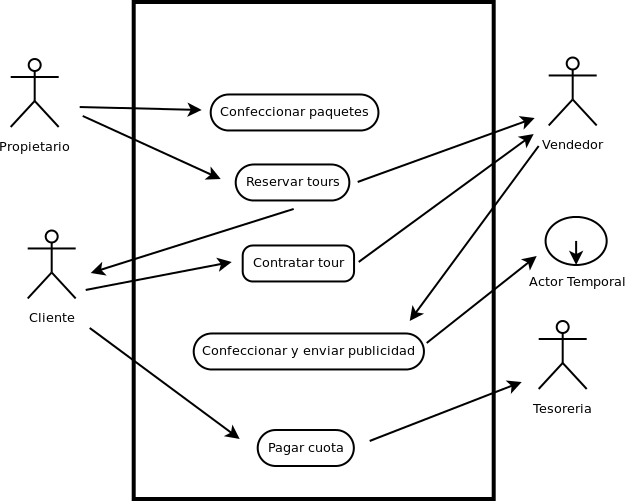
\includegraphics[width=1.0\textwidth]{diagramaCasosDeUso}}
\label{fig:celda}
\end{figure}
 
 
 
\section{Modelos de clases}

Diagramas de clases  
 
 

\end{document}